\section{Project Analysis} \label{analysis}

\subsection{A Brief Introduction to Fractals}

A fractal is ``a curve or geometrical figure, each part of which has the same statistical character as the whole''\cite{soanes_hawker_2013}.

Some fractals are defined by simple equations which exhibit chaotic behaviour. Arguably the most famous fractal, the Mandelbrot Set, is defined by the iterative equation, where \(Z_0=0+0i\), and \(C\) is the initial value in the complex plane.

\begin{equation*}
	Z_{n+1} = Z_n^2 + C \quad:\quad Z_n, c \in \mathbb{C}		
\end{equation*}

For a given point \(C\) to be in the Mandelbrot Set, the value of \(Z_n\) must remain bounded (i.e. not diverge to infinity) after the iterative series is repeated infinitely many times. This approach is used in most iterative fractal equations.

\vspace{0.5cm}

\begin{figure}[h]
	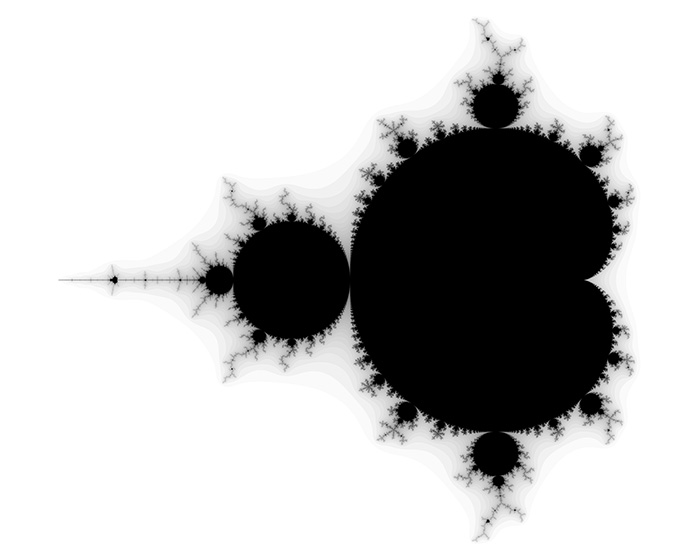
\includegraphics[scale=0.45]{mandelbrot.jpg}
	\caption{The standard Mandelbrot fractal\cite{bourke_2002}}
\end{figure}

Additionally, fractal variations can be created by changing the generating equation slightly. For example, changing the \(r\) in the Mandelbrot equation (\(Z_{n+1}=Z_n^r+C\)) yields the following fractals.

\begin{figure} [htp]
	\centering
	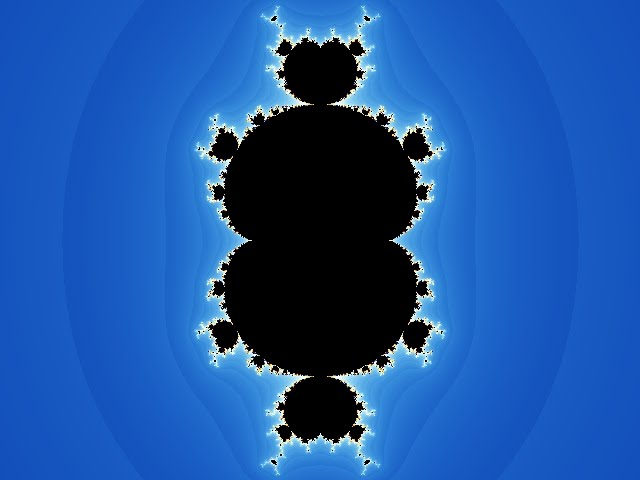
\includegraphics[width=.3\textwidth]{MsetOrder3.jpg}\hfill
	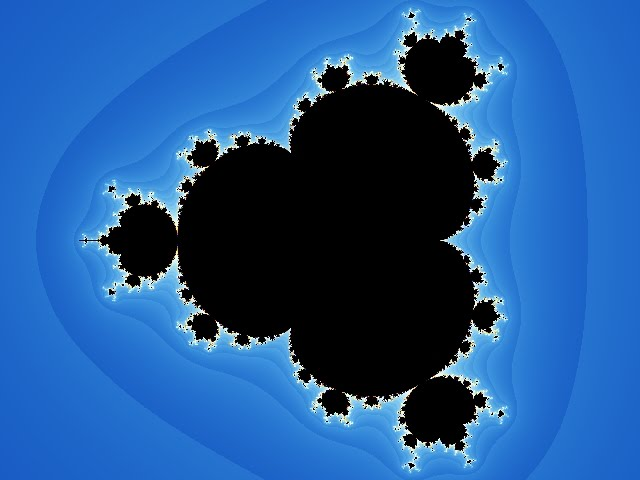
\includegraphics[width=.3\textwidth]{MsetOrder4.jpg}\hfill
	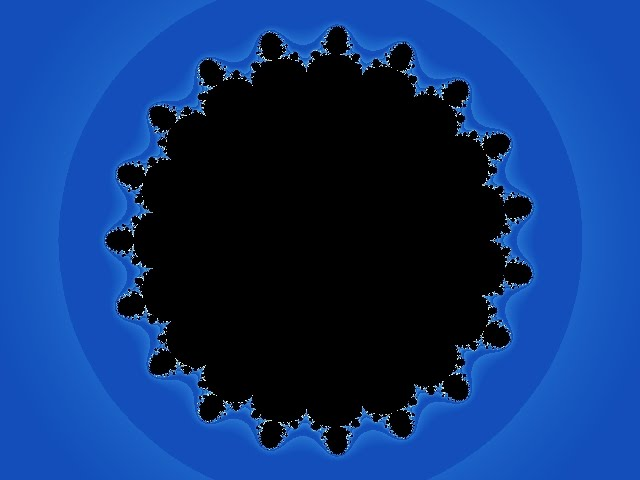
\includegraphics[width=.3\textwidth]{MsetOrder20.jpg}
	
	\caption{(left) \(r=3\), (centre) \(r=4\), (right) \(r=20\)}
\end{figure}

Other famous fractals include the Sierpiński Triangle, the Julia Set, Hilbert Spirals, etc. All are defined either by infinitely-recursive self-similar patterns or repeated equations.

\begin{figure}[htp]
	\centering
	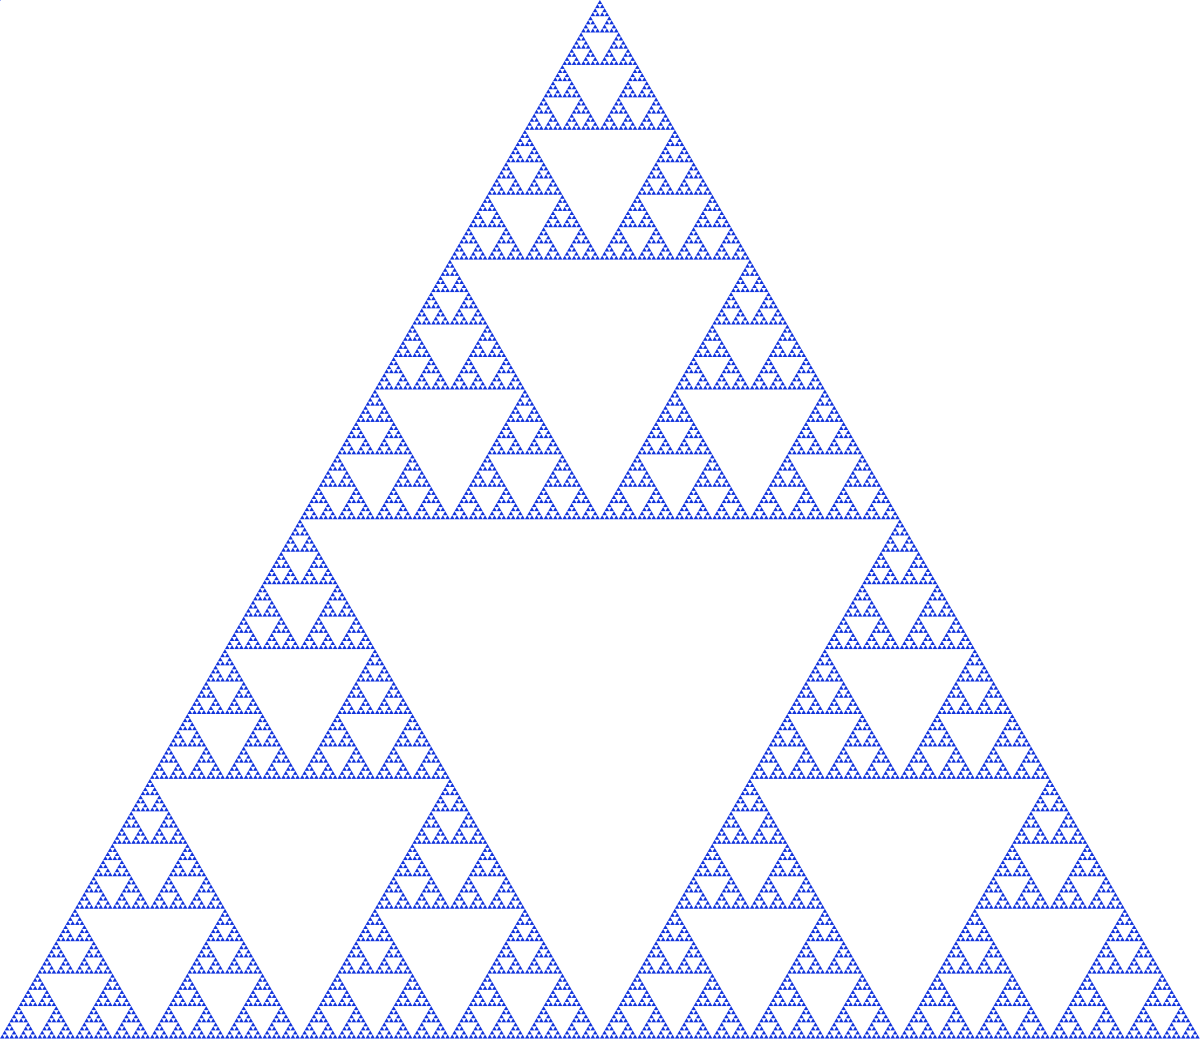
\includegraphics[width=.3\textwidth]{sierpinski-triangle.png}\hfill
	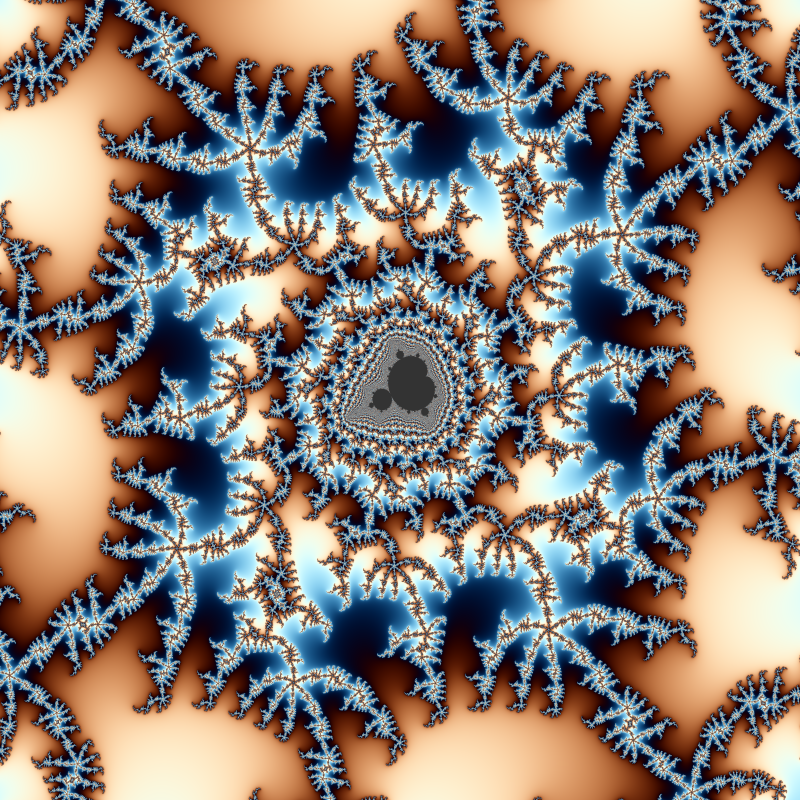
\includegraphics[width=.3\textwidth]{mandelbrot-zoom.png}\hfill
	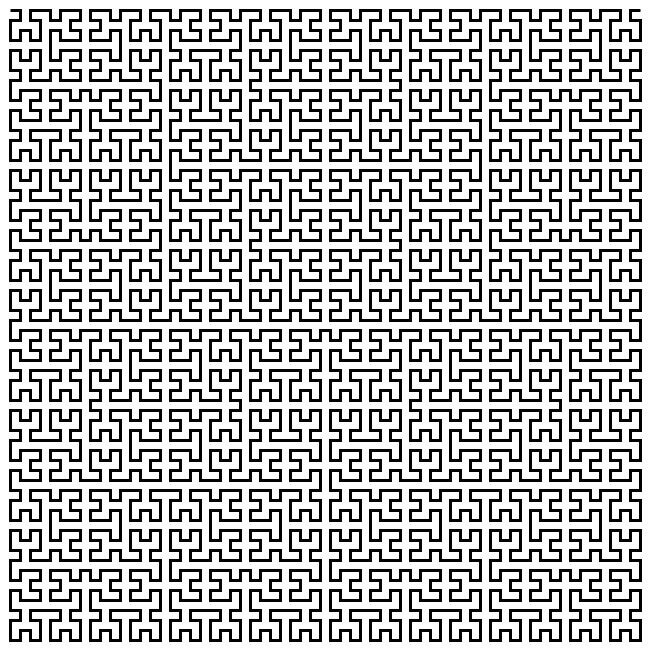
\includegraphics[width=.3\textwidth]{hilbert-curve.png}
	
	\caption{(left) Sierpiński-Triangle, (centre) Part of the Mandelbrot Set, (right) Hilbert Curve}
\end{figure}

\subsection{Defining the Problem}

Fractals have been the subject of much debate and curiosity throughout history, but, due to the computational requirements of generating them, research into them was very limited until the rise of the electronic computer.

The newfound levels of processing power allowed increasingly detailed images to be generated, and mathematicians were able to better understand the underlying equations and seemingly chaotic nature of fractals.

With the power of modern computers, it is possible to render some fractals in real-time and explore them to great depths, though there are still technical, physical and monetary hurdles to clear.

Many fractal rendering program exist online, however the majority of these are incomplete, inefficient applications that are not designed for high-performance and high zoom factors. While there are high-quality applications out there, the best ones are often quite expensive, making them inaccessible to the majority of potential-users. For example, some extremely advanced software costs almost \(\pounds 80\)\cite{slijkerman_2022}.

\begin{multicols}{2}
	
\paragraph{Technological Limitations} The further you zoom into a fractal, smaller the numbers you have to deal with. At lower zoom levels, this doesn't pose much of an issue, as \SI{64}{\bit} or even \SI{32}{\bit} floating point numbers often have the required precision to accurately render an image. At higher zoom levels, however, the precision of the numbers used starts to affect the image quality.

When zoomed in far enough, floating point rounding errors start to cause certain pixel positions to merge into one, causing unattractive ``blocky'' patterns in the image. Eventually, these blocks will consume the entire image and no more detail can be seen.

To get around this, it is possible to use high-precision floating point data types, though, since these are processed in software, not hardware, they are orders of magnitude slower than normal number types, and this can make the rendering process impractically slow.

Certain approaches can be taken to optimise the performance of high-performance number types. For example, it can be proven that \(Z_n\) will diverge to infinity if \(|Z_n|>2\) at any point. Additionally, advanced algorithms can mix fixed and multi-precision arithmetic to decrease the number of arithmetic operations that take place in software.

\paragraph{Program Limitations} Many fractal renderers do just that; render fractals. They don't support any kind of render export and do not allow for saving or reloading render configurations. 

Some programs have methods to save the rendered fractals as image files, but often have limiting export settings and don't support many resolutions. A wider range of programs allow the current position and zoom level, among other information, to be exported in a file. This allows the configuration to be reloaded and interesting locations in fractals to be shared easily.

\paragraph{Precision vs Performance} To increase rendering performance, most implementations of fractal renderers use strictly 32- or 64-bit floating point numbers. Since these data types are operated on directly by the hardware, they are extremely efficient. Unfortunately, 64-bit floating point values can only represent around 15 decimal places accurately, so zooming in far enough will exceed this precision and cause visual glitches.

To circumvent this issue, it is possible to use multi-precision floating point types that are capable of representing hundreds, thousands or even millions of bits, allowing for near-infinite zooms. These numbers, however, are implemented in software and are many orders of magnitude slower than standard floating point types.

For sufficiently optimised programs, it is possible, to a point, to use multi-precision floating point arithmetic, though the performance will be very poor.

Furthermore, some areas of different fractals require an immensely large number of iterations before a reasonable amount of detail can be obtained. A direct implication of this is that potentially millions of calculations must be done to determine the colour for a single pixel.

The two main issues above become even more extreme when combined with the goal of near-infinite zooming. Due to the nature of many fractals, the number of iterations required to get high levels of detail in areas close to the border of the fractal increases with zoom. Additionally, deeper zooms require higher precision numbers to accurately represent all the points. Combine these, and the result is an extremely slow, inefficient program which is not usable, in many cases.

\end{multicols}

\subsection{The End User}

A fast, fully-featured fractal viewer could be used by a wide range of people for a variety of different purposes.

Firstly, maths teachers could use the program to assist in their lessons, as well as providing students with an interactive resource to help with homework and to further their understanding.

Secondly, if the renderer is fast and precise, even at extremely high zoom levels, then it could be used by people researching fractals and examining their properties.

Finally, such a program could also be used by anyone who enjoys looking at fractals, which, most likely, provides a larger audience than the other users combined.

Combining these different user-bases, an efficient, intuitive fractal renderer could be used by a significant number of people for a broad spectrum of different purposes.

\vspace{0.5cm}

\begin{greenbox}{User Requirements}
	Unfortunately, each of the identified user groups will have a different set of specific requirements to be met. These will be covered later in the project, but it is likely that only a limited set of features can realistically be implemented.
\end{greenbox}

\subsection{Researching Existing Projects and User Requirements}

\pagebreak

There are many fractal viewers freely available online already, though almost all of them suffer from at least one very significant flaw:

\begin{enumerate}
	\item{Lack of precision}
	\item{Inadequate performance}
	\item{Insufficient customisability}
	\item{Limited file export options}
	\item{No ability to save configuration to a file}
\end{enumerate}

\vspace{0.5cm}

\begin{greybox}{Lack of precision}
	To increase performance, many simpler implementations use strictly 32- or 64-bit floating point values. Additionally, some implementations greatly reduce the number of samples run per pixel, meaning the fractal is lacking critical detail in some areas -- particularly those closest to the border of the fractal.
	
	\vspace{0.25cm}
	
	While it is possible to increase the maximum number of iterations run per pixel, moving from 64-bit (machine word) to multi-precision (software) floating point incurs a \emph{massive} performance hit, making it impractical in almost all cases.
\end{greybox}

\begin{greybox}{Inadequate performance}
	Many naive fractal renderers do not implement the necessary optimisations for the program to run at real-time with a native resolution. This links closely with the lack of precision, since the two are extremely closely related.
\end{greybox}

\begin{greybox}{Insufficient customisability}
	When rendering and exploring fractals there are a lot of settings that can change how it appears. For example, you can change the maximum number of iterations to allow, or the settings/algorithm for colouring the fractal.
	
	\vspace{0.25cm}
	
	Unfortunately, the vast majority of programs limit the customization of the fractal to the gradient used to colour it, not allowing the user to change any other settings.
	
	\vspace{0.25cm}
	
	Being able to change the most fundamental settings of the renderer allows for anyone using the software to gain a more intuitive understanding of both the fractal itself and the program.
\end{greybox}

\begin{greybox}{Limited file export options}
	A surprising number of fractal rendering programs do not allow the final product to be saved to a file, which is a nice feature to have if you want to examine them further in more software, for example.
	
\end{greybox}

\begin{greybox}{The ability to save configurations}
	Often, when exploring fractals, you come across areas of particular interest and would like to be able to return to that exact place in the future.
	
	\vspace{0.25cm}
	
	Very few programs actually implement this feature, and it is one which could be very useful in some circumstances.
\end{greybox}

\vspace{0.25cm}

\subsection{The End User}

A fast, fully-featured fractal viewer could be used by a wide range of people for a variety of different purposes.

Firstly, maths teachers could use the program to assist in their lessons, as well as providing students with an interactive resource to help with homework and to further their understanding.

Secondly, if the renderer is fast and precise, even at extremely high zoom levels, then it could be used by people researching fractals and examining their properties.

Finally, such a program could also be used by anyone who enjoys looking at fractals, which, most likely, provides a larger audience than the other users combined.

Combining these different user-bases, an efficient, intuitive fractal renderer could be used by a significant number of people for a broad spectrum of different purposes.

\vspace{0.5cm}

\begin{greenbox}{User Requirements}
	Unfortunately, each of the identified user groups will have a different set of specific requirements to be met. These will be covered later in the project, but it is likely that only a limited set of features can realistically be implemented.
\end{greenbox}

\subsection{Researching Existing Projects and User Requirements}

Look at online renderers (including Google's one??)
Look at offline renderers.

Pick out the best features

Talk to Josh
Talk to teachers
Talk to family

Identify the overarching requirements
Identify things that would be nice to have, but not necessarily required

\begin{codebox}{Test Box}
	\begin{lstlisting}[language=c++]
		#include<iostream>
		
		int main() {
			std::cout << "Hello, World\n";
			return 0;
		}
	\end{lstlisting}	
\end{codebox}

\begin{redbox}{Details Gathered -- TEMPORARY}
	Online Renderer
	\begin{enumerate}
		\item {	\href{https://math.hws.edu/eck/js/mandelbrot/MB.html}{https://math.hws.edu/eck/js/mandelbrot/MB.html} }
		\item { Rectangle zoom box is AWFUL }
		\item { Settings are useful }
		\subitem { Adjustable resolution }
		\subitem { Number of threads }
		\subitem { Palette editor }
		\subitem { Configuration Export }
		\subitem { Offers multiprecision floating point }
	\end{enumerate}
	
	XaoS Renderer
	\begin{enumerate}
		\item {	\href{https://fractalfoundation.org/resources/fractal-software/}{https://fractalfoundation.org/resources/fractal-software/} }
		\item { Method of moving around is quite clunky }
		\item { Almost every setting can be changed, which is good }
		\item { Multiple fractals supported }
		\item { Different colouring and shading options }
		\item { Some VERY interesting algorithms at play for performance boosts }
		\subitem { Some form of data retention between frames }
		\subitem { Progressive rendering }
		\subitem { Looks like a 128-bit float but no true multiprecision floating point }
		\subitem { Multiple approximations followed by progressive refining of the fractal }
		
		
		% \item { \href{https://mathr.co.uk/blog/2013-04-01_interior_coordinates_in_the_mandelbrot_set.html}{https://mathr.co.uk/blog/2013-04-01_interior_coordinates_in_the_mandelbrot_set.html} }
		
		% \item{ \href{chrome-extension://efaidnbmnnnibpcajpcglclefindmkaj/https://mathr.co.uk/mandelbrot/perturbation.pdf}{chrome-extension://efaidnbmnnnibpcajpcglclefindmkaj/https://mathr.co.uk/mandelbrot/perturbation.pdf} }
		
		% \item { \href{https://fractaltodesktop.com/perturbation-theory/index.html}{https://fractaltodesktop.com/perturbation-theory/index.html} }
		
		% \item{ \href{https://www.ultrafractal.com/whatsnew.html}{https://www.ultrafractal.com/whatsnew.html}}
	\end{enumerate}
	
\end{redbox}
